\documentclass{standalone}
\usepackage{tikz}
\usetikzlibrary{spy}

\begin{document}
\centering

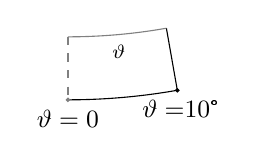
\begin{tikzpicture}[spy using outlines]
\def\theta{10}
\def\r{8}
\def\s{0.9}
\def\i{1.03}
\draw [domain=270:{270+\theta}] plot ({\r*cos(\x)}, {\r*sin(\x)});
\draw[gray,dashed] (270:\s*\r cm) -- (270:\r cm);
\draw ({270+\theta}:\s*\r cm) -- ({270+\theta}:\r cm);
\draw [gray,domain=270:{270+\theta}] plot ({\s*\r*cos(\x)}, {\s*\r*sin(\x)});
\draw ({270+\theta/2}:{\s*\r*\i cm}) node {\scriptsize{$\vartheta$}};
\filldraw ({270+\theta}:\r cm) circle(0.6pt);
\filldraw[gray] (270:\r cm) circle(0.6pt);
\draw (270:{\i*\r cm}) node {\small{$\vartheta=0°$}};
\draw ({270+\theta}:{\i*\r cm}) node {\small{$\vartheta=$}\theta°};
\end{tikzpicture}

\medskip

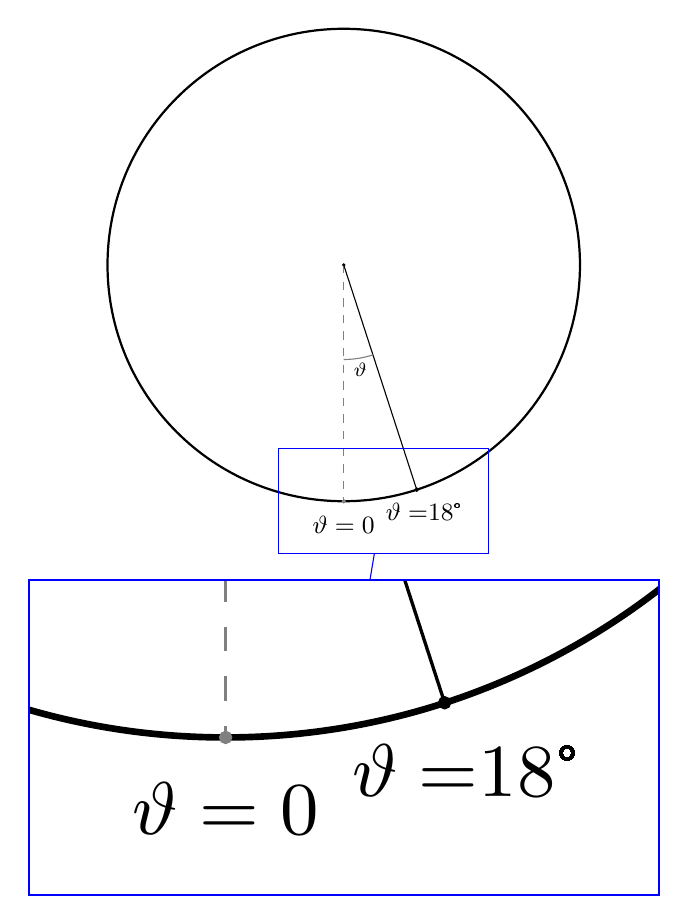
\begin{tikzpicture}[spy using outlines]
\def\theta{18}
\def\r{3}
\draw[thick] (0,0) circle(\r cm);
\draw (0,0) circle(0.4pt);
\draw[gray,dashed] (0cm,0cm) -- (270:\r cm);
\draw (0cm,0cm) -- ({270+\theta}:\r cm);
\draw [gray,domain=270:{270+\theta}] plot ({0.4*\r*cos(\x)}, {0.4*\r*sin(\x)});
\draw ({270+\theta/2}:0.45*\r cm) node {\scriptsize{$\vartheta$}};
\filldraw ({270+\theta}:\r cm) circle(0.6pt);
\filldraw[gray] (270:\r cm) circle(0.6pt);
\draw (270:1.1*\r cm) node {\small{$\vartheta=0°$}};
\draw ({270+\theta}:1.1*\r cm) node {\small{$\vartheta=$}\theta°};
\spy [blue,draw,height=4cm,width=8cm,magnification=3,connect spies] on (0.5,-3) in node at (0,-6);
\end{tikzpicture}

\end{document}